
\chapter{Fundamentação Teórica}
\label{chap:fundam}
Neste capítulo será discutido na seção 2.1, algumas das ferramentas que já se propõe a realizar
a comparação de moléculas, assim como alguns dos algoritmos que podem ser utilizados na 
análise de similaridade molecular que serão apresentados na seção 2.3, sendo que parte desses 
algoritmos já estão adaptados em algumas das ferramentas a serem apresentadas.
Também será exposto na seção 2.2 algumas formas de representação de uma molécula em um 
ambiente computacional, e sua importância para escolha de qual método de comparação de 
moléculas deverá ser utilizado.
\newpage
\section{FERRAMENTAS PARA COMPUTAÇÃO DE SIMILARIDADE MOLECULAR}

Devido a importância das ferramentas computacionais no processo de descobertas de fármacos, há diversos esforços dedicados ao desenvolvimento destas ferramentas, tornando-as cada vez mais eficientes e eficazes. Como resultado desses esforços, já se encontram disponíveis alguns sistemas computacionais que aplicam algoritmos de similaridade, realizam busca em bancos de dados, predição de propriedades físico-químicas e atividades biológicas, entre outras diversas funcionalidades importantes na pesquisa e desenvolvimento de fármacos. Esses softwares diferenciam-se de acordo com o custo de sua licença, funcionalidades implementadas, formatos de moléculas aceitos, representação computacional da molécula, método de computação de similaridade molecular, entre outros aspectos.

Uma das ferramentas populares entre pesquisadores na área de química medicinal é o ZINC. O sistema web ZINC é uma ferramenta livre que fornece para o usuário um banco de dados com mais de 21 milhões de estruturas catalogadas \cite{irwin2005zinc}. Além disso, o sistema armazena diversas informações  sobre cada molécula como : massa molecular, centros quirais, coeficiente de partição água-etanol calculado (cLogP). O ZINC armazena estruturas em formatos 2D, tal como o formato Simplified Molecular Input Line Entry System (SMILES), que são representações lineares utilizando uma sequência de caracteres para representação da estrutura molecular \cite{kumar2012}. Além do formato SMILES, o ZINC também aceita como formatos de entradas, Structure Data Format (SDF) e MOL2. O ZINC implementa rotinas para triagem virtual em sua base de dados utilizando os conceitos de similaridade molecular, permitindo ao pesquisador selecionar o grau de similaridade mínimo desejado, e retornando todas as moléculas em seu catálogo (banco de dados) com grau de similaridade igual ou superior ao selecionado pelo usuário \cite{irwin2005zinc}.

Outra ferramenta que pode ser utilizada para a comparação de similaridade entre moléculas é o software ANACONDA. Tal sistema realiza a computação da similaridade entre duas moléculas através da comparação de propriedades de suas respectivas superfícies moleculares utilizando projeção gnomônica . O emprego deste método permite	 a comparação de forma interativa de dois componentes, podendo sugerir modos de superposição entre as moléculas, e assim uma possível geração de um modelo famacofórico \cite{devillers1996}. Esta ferramenta apesar de apresentar bons resultados na comparação de similaridade molecular, não permite a comparação de mais de duas moléculas por consulta, e além disso também não fornece ao pesquisador nenhuma ferramenta para construção, ou manipulação de um banco de dados para catalogação das suas moléculas de estudo, exigindo assim um esforço para o mesmo catalogar suas moléculas de interesse, e realizar uma computação praticamente serial de similaridade entre moléculas que deseja-se estudar 

Utilizando uma abordagem para computação de similaridade molecular baseada na comparação de campos elestrostáticos e de campos de volume esférico, \cite{mestres1997mimic} descrevem um software denominado MIMIC, que implementa rotinas para realização de triagem virtual baseada na comparação de similaridade molecular. Este software permite ao pesquisador obter um índice de similaridade de alta precisão, pois consegue levar em consideração, além da estrutura da molécula, a contribuição de cada átomo na computação da similaridade molecular. Assim como descrito por \cite{devillers1996}, o MIMIC não realiza manipulação de banco de dados, por tanto necessita que o pesquisador insira as moléculas que deseja comparar na entrada do sistema de forma serial. Dessa maneira, para criar um banco de dados para catalogo de moléculas, o usuário necessita utilizar uma outra ferramenta para manipular bancos de dados, o que nem sempre é conveniente para um pesquisador que possua muitas moléculas para estudo, e que por muitas vezes não possui conhecimentos avançados de computação para fazer tal catalogação por conta própria.

Os esforços para implementação de ferramentas computacionais para cálculo de similaridade molecular não se restringem a programas de computador e/ou web sites. Alguns pesquisadores já tem desenvolvido bibliotecas multi-plataformas, capazes de interagir com várias linguagens de programação, e que implementam não somente rotinas para manipulação de moléculas em geral, mas também implementam algoritmos para computação de similaridade molecular. Nessa perspectiva, a Indigo Toolkit surge como uma das bibliotecas de acesso livre mais completas. Desenvolvida pela GGASoftware, e atualmente mantida pelo epam lifescience, Esta ferramenta é capaz de manipular os principais formatos disponíveis para representação de moléculas como: SMILES, SDF, Molfile, entre outros \cite{pavlov2011indigo}. O conjunto de ferramentas disponibilizado por essa biblioteca, permite ao usuário manipular moléculas, computar similaridade, buscar sub-estruturas e reações. A API indigo é capaz de utilizar diversos tipos de descritores moleculares, desde SMILES, até fingerprints (sequência de bits que representa presença ou ausência de uma determinada característica estrututral) e comparando moléculas através de diversas métricas como: coeficiente de Tanimoto, métrica euclidiana, e métrica de Tversky. Para sua utilização é necessário que esta biblioteca seja incorporada a um programa, que pode ser escrito em C/C++, java ou python. Esta biblioteca é utilizada na implementação do NatProDB, conforme será discutido posteriormente.

Utilizando uma abordagem de busca farmacofórica, O Pharmer é considerada uma ferramenta bastante robusta, e já tem sido utilizada até mesmo pelo Zinc no processo de triagem de moléculas similares em seu banco de dados \cite{koes2011pharmer}. O grande diferencial dessa ferramenta é a valocidade de processamento e computação de similaridade molecular em grandes bases de dados, chegando a ser uma ordem de magnitude mais rápido que as ferramentas computacionais já existentes \cite{koes2011pharmer}. O motivo para tal desempenho reside no fato de que em detrimento das demais ferramentas para triagem em bancos de dados moleculares através de modelos famacofóricos (que normalmente realizam a comparação serial de todas as moléculas de sua base de dados), o Pharmer utiliza uma estrutura de organização dados adaptada, denominada Pharmer KDB-tree data structure, e implementa um método de compração baseado em técnicas de computação visual: hashing geométrico e transformada generalizada de Hough. Através da utilização de tais tecnicas, o sistema não somente reduz o custo computacional para comparação de moléculas (grau de similaridade de modelos farmacofóricos), mas também reduz o tempo necessário para consulta no banco uma vez que a estrutura organizacional dos dados em sua base permite um direcionamento do sistema para alvos com maior probabilidade de serem similares.

\section{DESCRITORES MOLECULARES}
O descritor molecular pode ser considerado como o resultado da aplicação de procedimentos lógicos e matemáticos que transformam uma representação química codificada, em uma representação simbólica de uma molécula, em um formato padrão ou resultado de algum experimento padronizado, de forma a facilitar a manipulação dessas estruturas \cite{todeschini2008handbook}. Para o presente trabalho, o descritor molecular consiste no formato sobre o qual uma molécula é representada computacionalmente, e tal formato é importante para a computação de
similaridade, pois o descritor molecular é considerado um fator determinante da métrica a ser
aplicada para cálculo da similaridade estrutural. Nesta seção será apresentado alguns
descritores mais utilizados por sistemas que calculam similaridade entre moléculas\apud{todeschini2008handbook}{koes2011pharmer}.


     

 

\begin{figure}[!htb]
	\centering
	\caption[Exemplo de uma figura]{Exemplo de uma figura onde aparece uma imagem sem nenhum significado especial.}
	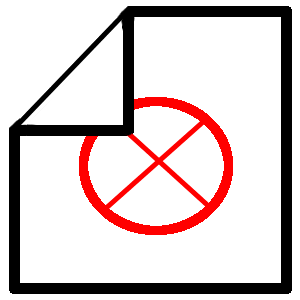
\includegraphics[width=0.2\textwidth]{dummy.png} % <- formatos PNG, JPG e PDF
	\fonte{ABNTEX, 2009\nocite{abnTeX2009}}
	\label{fig:dummy}
\end{figure}